\ifx\pdfminorversion\undefined\else\pdfminorversion=4\fi
\documentclass[aspectratio=169,t,xcolor=dvipsnames]{beamer}
%\documentclass[aspectratio=169,t,handout]{beamer}

% English version FAU Logo
\usepackage[english]{babel}
% German version FAU Logo
%\usepackage[ngerman]{babel}

\usepackage[utf8]{inputenc}
\usepackage[T1]{fontenc}
\usepackage{amsmath,amssymb}
\usepackage{graphicx}
\usepackage{listings}
\usepackage{url}
\usepackage{enumitem}
\usepackage{hyperref}
\usepackage{fontawesome}
\usepackage{graphicx}
\usepackage{booktabs}
\usepackage{calc}
\usepackage{ifthen}
\usepackage{xcolor}
\usepackage{tabularx}
\usepackage{makecell}
\usepackage{tikz}
\usepackage{tikz}
\usepackage{tikz-cd}
\usepackage{verbatim}
\usepackage{pgfplots,pgfplotstable,pgf-pie}
\usepackage{filecontents}
\newcommand{\plots}{0.611201}
\newcommand{\plotm}{2.19882}
\pgfplotsset{height=4cm,width=8cm,compat=1.16}
\pgfmathdeclarefunction{gauss}{2}{%
  \pgfmathparse{1/(#2*sqrt(2*pi))*exp(-((x-#1)^2)/(2*#2^2))}%
}

\tikzset{
    vertex/.style = {
        circle,
        fill            = black,
        outer sep = 2pt,
        inner sep = 1pt,
    }
}

\tikzset{
    mynode/.style={
        draw,
        thick,
        anchor=south west,
        minimum width=2cm,
        minimum height=1.3cm,
        align=center,
        inner sep=0.2cm,
        outer sep=0,
        rectangle split,
        rectangle split parts=2,
        rectangle split draw splits=false},
    reverseclip/.style={
        insert path={(current page.north east) --
            (current page.south east) --
            (current page.south west) --
            (current page.north west) --
            (current page.north east)}
    }
}

\tikzset{basic/.style={
        draw,
        rectangle split,
        rectangle split parts=2,
        rectangle split part fill={blue!20,white},
        minimum width=2.5cm,
        text width=2cm,
        align=left,
        font=\itshape
    },
    Diamond/.style={ diamond,
                      draw,
                      shape aspect=2,
                      inner sep = 2pt,
                      text centered,
                      fill=blue!10!white,
                      font=\itshape
                    }}


\tikzset{level 1/.append style={sibling angle=50,level distance = 165mm}}
\tikzset{level 2/.append style={sibling angle=20,level distance = 45mm}}
\tikzset{every node/.append style={scale=1}}

\usetikzlibrary{arrows,decorations.pathmorphing,backgrounds,fit,positioning,shapes.symbols,chains,intersections,snakes,positioning,matrix,mindmap,shapes.multipart,shapes,calc,shapes.geometric}

% read in data file


\newcommand{\MaxNumberX}{3}
\newcommand{\MaxNumberY}{5}
\newcommand{\tikzmark}[1]{\tikz[remember picture] \node[coordinate] (#1) {#1};}

\pgfplotstableread{data/iris.dat}\iris
\pgfplotstablegetrowsof{\iris}
\pgfplotsset{compat=1.14}
\pgfmathsetmacro\NumRows{\pgfplotsretval-1}
\definecolor{airforceblue}{rgb}{0.36, 0.54, 0.66}

\usepgfplotslibrary{groupplots}
% Options:
%  - inst:      Institute
%                 med:      MedFak FAU theme
%                 nat:      NatFak FAU theme
%                 phil:     PhilFak FAU theme
%                 rw:       RWFak FAU theme
%                 rw-jura:  RWFak FB Jura FAU theme
%                 rw-wiso:  RWFak FB WISO FAU theme
%                 tf:       TechFak FAU theme
%  - image:     Cover image on title page
%  - plain:     Plain title page
%  - longtitle: Title page layout for long title
\usetheme[%
  image,%
  longtitle,%
  tf
]{fau}

% Enable semi-transparent animation preview
\setbeamercovered{transparent}


\lstset{%
  language=Python,
  tabsize=2,
  basicstyle=\tt,
  keywordstyle=\color{blue},
  commentstyle=\color{green!50!black},
  stringstyle=\color{red},
  numbers=left,
  numbersep=0.5em,
  xleftmargin=1em,
  numberstyle=\tt
}


% Title, authors, and date
\title[KDD]{Chapter VII: Cluster analysis}
\subtitle{Knowledge Discovery in Databases}
\author[L.~Melodia]{Luciano Melodia M.A.}
% English version
\institute[Department]{Evolutionary Data Management, Friedrich-Alexander University Erlangen-Nürnberg}
% German version
%\institute[Lehrstuhl]{Lehrstuhl, Friedrich-Alexander-Universit\"at Erlangen-N\"urnberg}
\date{Summer semester 2021}
% Set additional logo (overwrites FAU seal)
%\logo{\includegraphics[width=.15\textwidth]{themefau/art/xxx/xxx.pdf}}
\begin{document}
  % Title
  \maketitle

  {
    \setbeamertemplate{footline}{}
    \begin{frame}{Chapter VII: Cluster analysis}
        \begin{itemize}
            \item \textbf{Cluster analysis: basic concepts.}
            \item Partitioning methods.
            \item Hierarchical methods.
            \item Density-based methods.
            \item Grid-based methods.
            \item Evaluation of clustering.
            \item Summary.
        \end{itemize}
    \end{frame}
  }

  {
    \setbeamertemplate{footline}{}
    \begin{frame}{What is cluster analysis?}
        \begin{itemize}
          \item \textbf{{\color{airforceblue}Cluster}: A collection of data objects within a larger set that are.}
          \begin{itemize}
            \item {\color{airforceblue}Similar (or related)} to one another within the same group and,
            \item dissimilar (or unrelated) to the objects outside the group.
          \end{itemize}
          \item \textbf{{\color{airforceblue}Cluster analysis} (or clustering, data segmentation, $\ldots$).}
          \begin{itemize}
            \item {\color{airforceblue}Define similarities} among data based on the characteristics found in the data (input from user!).
            \item Group similar data objects into clusters.
          \end{itemize}
          \item \textbf{Unsupervised learning:}
          \begin{itemize}
            \item No predefined classes.
            \item I.e., learning by observation (vs. learning by examples: supervised).
          \end{itemize}
          \item \textbf{Typical applications:}
          \begin{itemize}
            \item As a stand-alone tool to get insight into data distribution.
            \item As a preprocessing step for other algorithms.
          \end{itemize}
        \end{itemize}
    \end{frame}
  }

  {
    \setbeamertemplate{footline}{}
    \begin{frame}{Clustering for data understanding and applications}
        \begin{itemize}
          \item \textbf{Biology:}
          \begin{itemize}
            \item Taxonomy of living things: kingdom, phylum, class, order, family, genus, and species.
          \end{itemize}
          \item \textbf{Information retrieval:}
          \begin{itemize}
            \item Document clustering.
          \end{itemize}
          \item \textbf{Land use:}
          \begin{itemize}
            \item Identification of areas of similar land use in an earth-observation database.
          \end{itemize}
          \item \textbf{Marketing:}
          \begin{itemize}
            \item Help marketers discover distinct groups in their customer bases, and then use this knowledge to develop targeted marketing programs.
          \end{itemize}
          \item \textbf{City planning:}
          \begin{itemize}
            \item Identifying groups of houses according to their house type, value, and geographical location.
          \end{itemize}
          \item \textbf{Earthquake studies:}
          \begin{itemize}
            \item Observed earthquake epicenters should be clustered along continent faults.
          \end{itemize}
          \item \textbf{Climate:}
          \begin{itemize}
            \item Understanding earth climate, find patterns of atmosphere and ocean.
          \end{itemize}
        \end{itemize}
    \end{frame}
  }

  {
    \setbeamertemplate{footline}{}
    \begin{frame}{Quality: what is good clustering?}
        \begin{itemize}
          \item \textbf{A good clustering method will produce high-quality clusters.}
          \begin{itemize}
            \item \textbf{\color{airforceblue}High intra-class similarity:}
            \begin{itemize}
              \item Cohesive within clusters.
            \end{itemize}
            \item \textbf{\color{airforceblue}Low inter-class similarity:}
            \begin{itemize}
              \item Distinctive between clusters.
            \end{itemize}
          \end{itemize}
          \item \textbf{The {\color{airforceblue}quality} of a clustering method depends on:}
          \begin{itemize}
            \item the \textbf{\color{airforceblue}similarity measure} used by the method,
            \item its implementation, and
            \item its ability to discover some or all of the hidden patterns.
          \end{itemize}
        \end{itemize}
    \end{frame}
  }

  {
    \setbeamertemplate{footline}{}
    \begin{frame}{Measure the quality of clustering}
        \begin{itemize}
          \item \textbf{Dissimilarity/similarity metric:}
          \begin{itemize}
            \item Similarity is expressed in terms of a distance function, typically a metric: $d(x,y)$.
            \item The definitions of distance functions are usually rather different for interval-scaled, Boolean, categorical, ordinal, ratio, and vector variables (see chapter 2).
            \item \textbf{\color{airforceblue}Weights} should be associated with different variables \\
                  based on applications and data semantics.
          \end{itemize}
          \item \textbf{Quality of clustering:}
          \begin{itemize}
            \item There is usually a separate \textbf{\color{airforceblue}"quality" function} that measures the "goodness" of a cluster.
            \item It is hard to define "similar enough" or "good enough."
            \item The answer is typically highly subjective.
          \end{itemize}
        \end{itemize}
    \end{frame}
  }

  {
    \setbeamertemplate{footline}{}
    \begin{frame}{Considerations for cluster analysis}
        \begin{itemize}
          \item \textbf{Partitioning criteria:}
          \begin{itemize}
            \item Single level vs. hierarchical partitioning.
            \item Often, multi-level hierarchical partitioning is desirable.
          \end{itemize}
          \item \textbf{Separation of clusters:}
          \begin{itemize}
            \item Exclusive (e.g., one customer belongs to only one region) vs.
            \item Non-exclusive (e.g., one document may belong to more than one class).
          \end{itemize}
          \item \textbf{Similarity measure:}
          \begin{itemize}
            \item Distance-based (e.g., Euclidian, road network, vector) vs.
            \item Connectivity-based (e.g., density or contiguity).
          \end{itemize}
          \item \textbf{Clustering space:}
          \begin{itemize}
            \item Full space (often when low-dimensional) vs.
            \item Subspaces (often in high-dimensional clustering).
          \end{itemize}
        \end{itemize}
    \end{frame}
  }

  {
    \setbeamertemplate{footline}{}
    \begin{frame}{Requirements and challenges}
        \begin{itemize}
          \item \textbf{Scalability:}
          \begin{itemize}
            \item Clustering all the data instead of only on samples.
          \end{itemize}
          \item \textbf{Ability to deal with different types of attributes:}
          \begin{itemize}
            \item Numerical, binary, categorical, ordinal, linked, and mixture of these.
          \end{itemize}
          \item \textbf{Constraint-based clustering:}
          \begin{itemize}
            \item User may give inputs on constraints.
            \item Use domain knowledge to determine input parameters.
          \end{itemize}
          \item \textbf{Interpretability and usability.}
          \item \textbf{Others:}
          \begin{itemize}
            \item Discovery of clusters with arbitrary shape.
            \item Ability to deal with noisy data.
            \item Incremental clustering and insensitivity to input order.
            \item High dimensionality.
          \end{itemize}
        \end{itemize}
    \end{frame}
  }

  {
    \setbeamertemplate{footline}{}
    \begin{frame}{Major clustering approaches}
        \begin{itemize}
          \item \textbf{Partitioning approach:}
          \begin{itemize}
            \item Construct various partitions and then evaluate them by some criterion.
            \item E.g., minimizing the sum of square errors.
            \item Typical methods: k-means, k-medoids, CLARA, CLARANS.
          \end{itemize}
          \item \textbf{Hierarchical approach:}
          \begin{itemize}
            \item Create a hierarchical decomposition of the set of data (or objects) using some criterion.
            \item Typical methods: AGNES, DIANA, BIRCH, CHAMELEON.
          \end{itemize}
          \item \textbf{Density-based approach:}
          \begin{itemize}
            \item Based on connectivity and density functions.
            \item Typical methods: DBSCAN, OPTICS, DENCLUE.
          \end{itemize}
          \item \textbf{Grid-based approach:}
          \begin{itemize}
            \item Based on a multiple-level granularity structure.
            \item Typical methods: STING, WaveCluster, CLIQUE.
          \end{itemize}
        \end{itemize}
    \end{frame}
  }

  {
    \setbeamertemplate{footline}{}
    \begin{frame}{Major clustering approaches (II)}
        \begin{itemize}
          \item \textbf{Model-based approach:}
          \begin{itemize}
            \item A model is hypothesized for each of the clusters and tries to find the best fit of that model to each other.
            \item Typical methods: EM, SOM, COBWEB.
          \end{itemize}
          \item \textbf{Frequent-pattern-based approach:}
          \begin{itemize}
            \item Based on the analysis of frequent patterns.
            \item Typical methods: p-Cluster.
          \end{itemize}
          \item \textbf{User-guided or constraint-based approach:}
          \begin{itemize}
            \item Clustering by considering user-specified or application-specific constraints.
            \item Typical methods: COD (obstacles), constrained clustering.
          \end{itemize}
          \item \textbf{Link-based clustering:}
          \begin{itemize}
            \item Objects are often linked together in various ways.
            \item Massive links can be used to cluster objects: SimRank, LinkClus.
          \end{itemize}
        \end{itemize}
    \end{frame}
  }

  {
    \setbeamertemplate{footline}{}
    \begin{frame}{Chapter VII: Cluster analysis}
        \begin{itemize}
            \item Cluster analysis: basic concepts.
            \item \textbf{Partitioning methods.}
            \item Hierarchical methods.
            \item Density-based methods.
            \item Grid-based methods.
            \item Evaluation of clustering.
            \item Summary.
        \end{itemize}
    \end{frame}
  }

  {
    \setbeamertemplate{footline}{}
    \begin{frame}{Partitioning algorithms: basic concept}
        \begin{itemize}
          \item \textbf{Partitioning method:}
          \begin{itemize}
            \item Partition a database $D$ of $n$ objects $o_j, j \in \{1, \ldots, n\}$ into a set of $k$-clusters $C_i$, $1 \leq i \leq k$ such that the sum of squared distances to $c_i$ is minimized \\ (where $c_i$ is the \textbf{\color{airforceblue}centroid} or \textbf{\color{airforceblue}medoid} of cluster $C_i$):
            \begin{align}
              \min \sum_{i=1}^{k} \sum_{o \in C_i} d(o,c_i)^2.
            \end{align}
          \end{itemize}
          \item \textbf{Given $k$, find a partition of $k$ clusters that optimizes the chosen partitioning criterion.}
          \begin{itemize}
            \item Globally optimal: exhaustively enumerate all partitions.
            \item Heuristic methods: k-means and k-medoids algorithms.
            \item \textbf{\color{airforceblue}k-means} (MacQueen'67, Lloyd'57/'82):
            \begin{itemize}
              \item Each cluster is represented by the center of the cluster.
            \end{itemize}
            \item \textbf{\color{airforceblue}k-medoids} or PAM (Partition around medoids) (Kaufman \& Rousseeuw'87):
            \begin{itemize}
              \item Each cluster is represented by one of the objects in the cluster.
            \end{itemize}
          \end{itemize}
        \end{itemize}
    \end{frame}
  }

  {
    \setbeamertemplate{footline}{}
    \begin{frame}{The $k$-means clustering method}
        \begin{itemize}
          \item \textbf{Given $k$, the $k$-means algorithm is implemented in four steps:}
          \begin{itemize}
            \item[1.] Partition the database into $k$ non-empty subsets.
            \begin{itemize}
              \item E.g. the first $\frac{n}{k}$ objects, then the next $\frac{n}{k}$ objects, $\ldots$
            \end{itemize}
            \item[2.] Compute the centroids of the \textbf{clusters} of the current partitioning.
            \begin{itemize}
              \item The centroid is the center, i.e. mean point, of the cluster.
              \item For each attribute (or dimension), calculate the average value.
            \end{itemize}
            \item[3.] Assign each object to the cluster with the nearest centroid.
            \begin{itemize}
              \item That is, for each object calculate distance to each of the $k$\\
              centroids and pick the one with the smallest distance.
            \end{itemize}
          \item[4.] If any object has changed its cluster, go back to step 2. Otherwise stop.
          \end{itemize}
          \item \textbf{Variant:}
          \begin{itemize}
            \item Start with arbitrarily chosen $k$ objects as initial centroids in step $1$.
            \item Continue with step $3$.
          \end{itemize}
        \end{itemize}
    \end{frame}
  }

  {
    \setbeamertemplate{footline}{}
    \begin{frame}{An example of $k$-means clustering}
      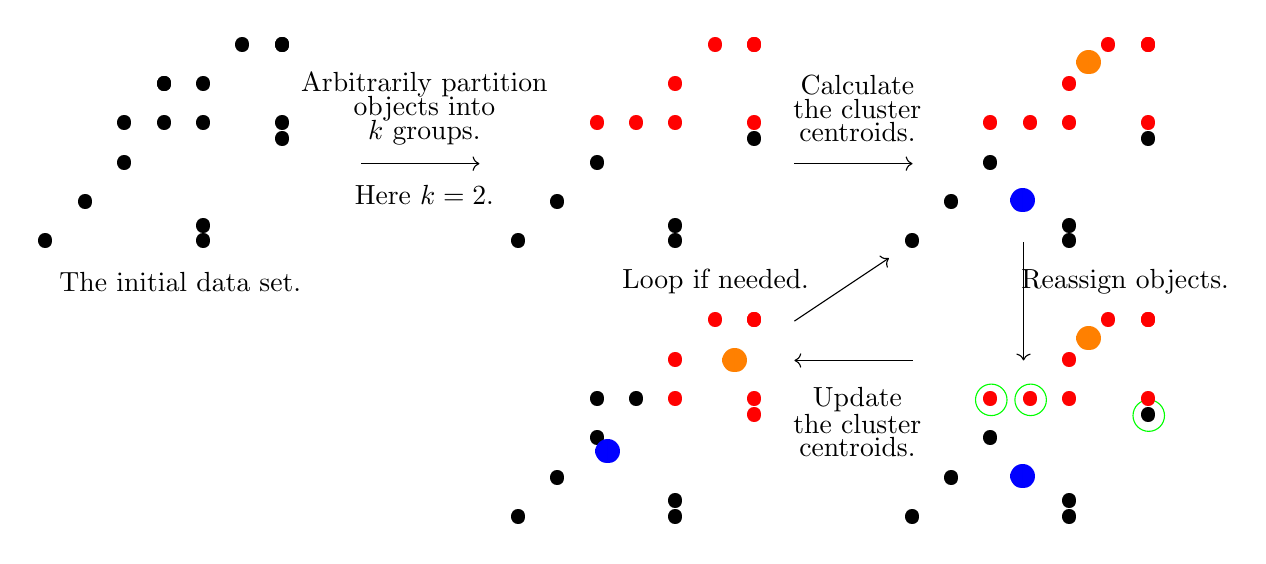
\begin{tikzpicture}
        \node [black] at (3,2.5) {\Large\textbullet};
        \node [black] at (4,3.5) {\Large\textbullet};
        \node [black] at (2,2.5) {\Large\textbullet};
        \node [black] at (2.5,3) {\Large\textbullet};
        \node [black] at (3,1) {\Large\textbullet};
        \node [black] at (3,1.2) {\Large\textbullet};
        \node [black] at (1,1) {\Large\textbullet};
        \node [black] at (1.5,1.5) {\Large\textbullet};
        \node [black] at (2,2) {\Large\textbullet};
        \node [black] at (2.5,2.5) {\Large\textbullet};
        \node [black] at (3,3) {\Large\textbullet};
        \node [black] at (3.5,3.5) {\Large\textbullet};
        \node [black] at (4,3.5) {\Large\textbullet};
        \node [black] at (4,2.3) {\Large\textbullet};
        \node [black] at (4,2.5) {\Large\textbullet};
        \node [black] at (2.5,3) {\Large\textbullet};
        \node [black] at (2.7,0.5) {The initial data set.};

        \node [black] at (7,1) {\Large\textbullet};
        \node [black] at (7.5,1.5) {\Large\textbullet};
        \node [black] at (8,2) {\Large\textbullet};
        \node [red] at (8,2.5) {\Large\textbullet};
        \node [red] at (8.5,2.5) {\Large\textbullet};
        \node [black] at (9,1) {\Large\textbullet};
        \node [black] at (9,1.2) {\Large\textbullet};
        \node [red] at (9,2.5) {\Large\textbullet};
        \node [red] at (9,3) {\Large\textbullet};
        \node [red] at (9.5,3.5) {\Large\textbullet};
        \node [red] at (10,3.5) {\Large\textbullet};
        \node [red] at (10,3.5) {\Large\textbullet};
        \node [black] at (10,2.3) {\Large\textbullet};
        \node [red] at (10,2.5) {\Large\textbullet};

        \node [black] at (12,1) {\Large\textbullet};
        \node [black] at (12.5,1.5) {\Large\textbullet};
        \node [black] at (13,2) {\Large\textbullet};
        \node [red] at (13,2.5) {\Large\textbullet};
        \node [red] at (13.5,2.5) {\Large\textbullet};
        \node [black] at (14,1) {\Large\textbullet};
        \node [black] at (14,1.2) {\Large\textbullet};
        \node [red] at (14,2.5) {\Large\textbullet};
        \node [red] at (14,3) {\Large\textbullet};
        \node [red] at (14.5,3.5) {\Large\textbullet};
        \node [red] at (15,3.5) {\Large\textbullet};
        \node [red] at (15,3.5) {\Large\textbullet};
        \node [black] at (15,2.3) {\Large\textbullet};
        \node [red] at (15,2.5) {\Large\textbullet};
        \node [orange] at (14.25,3.25) {\Huge\textbullet};
        \node [blue] at (13.41,1.5) {\Huge\textbullet};

        \node [black] at (12,-2.5) {\Large\textbullet};
        \node [black] at (12.5,-2) {\Large\textbullet};
        \node [black] at (13,-1.5) {\Large\textbullet};
        \node [red] at (13,-1) {\Large\textbullet};
        \node [red] at (13.5,-1) {\Large\textbullet};
        \draw[green] (13,-1) circle (0.2cm);
        \draw[green] (13.5,-1) circle (0.2cm);
        \node [black] at (14,-2.5) {\Large\textbullet};
        \node [black] at (14,-2.3) {\Large\textbullet};
        \node [red] at (14,-1) {\Large\textbullet};
        \node [red] at (14,-0.5) {\Large\textbullet};
        \node [red] at (14.5,0) {\Large\textbullet};
        \node [red] at (15,0) {\Large\textbullet};
        \node [red] at (15,0) {\Large\textbullet};
        \node [black] at (15,-1.2) {\Large\textbullet};
        \draw[green] (15,-1.2) circle (0.2cm);
        \node [red] at (15,-1) {\Large\textbullet};
        \node [orange] at (14.25,-0.25) {\Huge\textbullet};
        \node [blue] at (13.41,-2) {\Huge\textbullet};

        \node [black] at (7,-2.5) {\Large\textbullet};
        \node [black] at (7.5,-2) {\Large\textbullet};
        \node [black] at (8,-1.5) {\Large\textbullet};
        \node [black] at (8,-1) {\Large\textbullet};
        \node [black] at (8.5,-1) {\Large\textbullet};
        \node [black] at (9,-2.5) {\Large\textbullet};
        \node [black] at (9,-2.3) {\Large\textbullet};
        \node [red] at (9,-1) {\Large\textbullet};
        \node [red] at (9,-0.5) {\Large\textbullet};
        \node [red] at (9.5,0) {\Large\textbullet};
        \node [red] at (10,0) {\Large\textbullet};
        \node [red] at (10,0) {\Large\textbullet};
        \node [red] at (10,-1.2) {\Large\textbullet};
        \node [red] at (10,-1) {\Large\textbullet};
        \node [orange] at (9.75,-0.53) {\Huge\textbullet};
        \node [blue] at (8.14,-1.68) {\Huge\textbullet};

        \draw [->] (13.41,1) -- (13.41,-0.5);
        \node [black] at (14.7,0.5) {Reassign objects.};

        \draw [->] (5,2) -- (6.5,2);
        \node [black] at (5.8,3) {Arbitrarily partition};
        \node [black] at (5.8,2.7) {objects into};
        \node [black] at (5.8,2.4) {$k$ groups.};
        \node [black] at (5.8,1.6) {Here $k = 2$.};

        \draw [->] (10.5,2) -- (12,2);
        \node [black] at (11.3,3) {Calculate};
        \node [black] at (11.3,2.7) {the cluster};
        \node [black] at (11.3,2.4) {centroids.};

        \draw [->]  (12,-0.5) -- (10.5,-0.5);
        \draw [->]  (10.5,0)--(11.7,0.8);
        \node [black] at (9.5,0.5) {Loop if needed.};
        \node [black] at (11.3,-1) {Update};
        \node [black] at (11.3,-1.3) {the cluster};
        \node [black] at (11.3,-1.6) {centroids.};
      \end{tikzpicture}
    \end{frame}
  }

  { % Questions?
    \setbeamertemplate{footline}{}
    \begin{frame}[c]
      \begin{center}
        Thank you for your attention.\\
        {\bf Any questions about the seventh chapter?}\\[0.5cm]
        Ask them now, or again, drop me a line: \\
        \faSendO \ \texttt{luciano.melodia@fau.de}.
      \end{center}
    \end{frame}
  }
\end{document}
